\subsection{Användarbeskrivning}
\label{subsec:userdesc}

Vid utvecklingen av SuperRecorder för Android måste hänsyn tas till två olika användare. Den första är utvecklaren som ska integrera SDK:t i sin applikation och den andra är testaren som ska testa utvecklarens applikation med SuperRecorder.

\textbf{Utvecklaren} \\
Utveklaren kan förväntas ha god erfarenhet inom Androidutveckling. Den primära målgruppen för utvecklarna är de som har applikationutveckling som yrke men SDK:t kan även användas av de som vill testa en applikation som utvecklats på fritiden. Den senare målgruppen kan dock också antas ha goda kunskaper inom Androidutveckling. 

Det finns en önskan från The Beta Family att SDK:t ska kunna integreras i en existerande applikation på två minuter. Det är därför av vikt att integreringen av SDK:t görs så intuiv som möjligt för att tillgodose den önskan från uppdragsgivaren.

\textbf{Testaren} \\
Uppdragsgivaren är tydliga med att alla personer, oavsett kön eller ålder, ska kunna testa appar med SuperRecorder. Detta för att utvecklaren själv ska kunna välja vilken målgrupp som applikationen ska testas på. Testaren kan därför inte antas besitta djupare kunskap inom Android än daglig användning. Det är således av största vikt att det grafiska gränssnittet till SuperRecorden görs så användarvänlig som möjligt.

\textbf{Personas och scenarion} \\
För att alla i projektgruppen ska få en samlad bild av målgruppen har vi använt oss av personas och användarscenarios för att alla ska få en verklig bild av vem som kommer att använda slutprodukten och hur den kommer att användas. Dessa presenteras i nästa avsnitt.
\newpage	
\subsubsection{Persona - Patrik Berglind}

\vspace{40px}


\includegraphics[scale=0.4]{persona1.png}\\

\vspace{50px}

{\fontsize{1cm}{1em}\selectfont Patrik Berglind}

\vspace{20px}

\begin{tabular}{lllll}
  Ålder & \textbf{26} \\
  Relationsstatus & \textbf{Sambo} \\
  Arbete & \textbf{Applikationsutvecklare}\\
  Utbildning & \textbf{Yrkesutbildning applikationsprogrammering} \\
  Boende & \textbf{Kungsholmen} \\
\end{tabular}

\vspace{20px}

Patrik Berglind är 26 år gammal och uppvuxen i Kramfors. Efter att Patrik tagit examen från Yrkeshögskolan Höga Kusten för tre år sedan där han läste till applikationsprogrammerare flyttade han till Stockholm och har sedan dess arbetat på App AB. Patrik ingår i en liten projektgrupp där han fingerar som programmerare och utvecklar mobilapplikationer till både iPhone och Android. Patrik Berglinds stora passion är programmering och han har programmerat sedan han var 15 år. När Patrik skulle välja utbildning var yrkesutbildningen inom applikationsprogrammering ett självklart val eftersom han ville ut i arbetslivet snabbt med eftertraktad kompetens inom den expansiva appmarknaden och Patrik fick arbetet som applikationsutvecklare på App AB en vecka efter sin examen.

Patrik har på senare år utvecklats till en riktigt frilufsmänniska och brukar åka till norra Norge och vandra i bergen tillsammans med sin sambo Lisa med jämna mellanrum.

Patrik och Lisa väntar sitt första barn och går i tankarna att köpa ett radhus i någon förort till Stockholm. De har tittat extra mycket på ett radhus i Boo alldelse i närheten av Järlasjön och ett annat vid Sticklinge Udde.

\textbf{Mål}\\
Även fast Patrik älskar att programmera har han på sistone känt att det blir tradigt att bara programmera hela dagarna och har därför som mål att inom kort försöka bli projektledare och således själv få styra en projektgrupp.
\newpage

\subsubsection{Scenario 1 - Patrik Berglind}
Patrik har precis slagit sig ner i sin arbetsstol i det öppna kontorslandskapen på App AB och öppnat sin laptop. Han känner sig stressad eftersom han är sen till en visning av ett radhus i Åkersberga. Men innan han kan lämna kontoret för dagen måste han integrera SDK:t från TheBetaFamily i appen från Willys som hans projektgrupp arbetat med den senaste månaden och som nu är klar för betatestning.

Han skyndar sig in på The Beta Familys hemsida och laddar ner SDK:t till SuperRecorden och sparar ner den i Framworks-mappen i projektet. Han fortsätter sedan med att lägga till de bibliotek som krävs för att köra SuperRecorder. Han öppnar sedan projektet i Eclipse och lägger till den koden som angetts på The Beta Familys hemsida. När han är klar med detta kompilerar han projektet, avslutar eclipse och slår igen sin laptop innan han med långa kliv går mot bilen.
\newpage
\subsubsection{Persona - Emma Henriksson}

\vspace{40px}

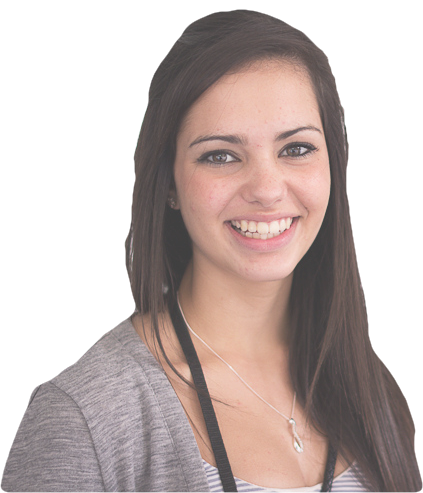
\includegraphics[scale=0.5]{persona2.png}\\

\vspace{50px}

{\fontsize{1cm}{1em}\selectfont Emma Henriksson}

\vspace{20px}

\begin{tabular}{lllll}
  Ålder & \textbf{18} \\
  Relationsstatus & \textbf{Singel} \\
  Sysselsättning & \textbf{Gymnasiestudent}\\
  Boende & \textbf{Täby} \\
\end{tabular}

\vspace{20px}
Emma Henriksson är 18 år gammal och pluggar teknik på Åva Gymnasium i Täby där hon går i tvåan. Emmas favoritämnen är matematik och fysik så det var aldrig någon tvekan om vilket gymnasieprogram hon skulle välja. Emma är sugen på att studera vidare direkt efter gymnasiet och hon står inför valet mellan KTH och Chalmers där hon vill plugga till Civilingenjör i Maskinteknik.

En av Emmas största intressen är film och hennes absoluta favoritfilm är La vita é bella. Om hon inte tittar på film lyssnar hon gärna på musik och då är det The National eller Sufjan Stevens som gäller. I övrigt lever hon ett vanligt tonårsliv där hon gärna umgås med vänner, både på riktigt och på Facebook.


\textbf{Mål}\\
Emmas mål är att komma in på ett civilingenjörsprogram på antingen KTH eller Chalmers. Inom den närmsta framtiden vill hon gärna hitta ett eget boende och hon drömmer om att få testa på att leva och bo utomlands.

\newpage

\subsubsection{Scenario 1 - Emma Henriksson}
Klockan är 7.30 och Emma har precis hoppat på bussen mot skolan. Eftersom hållplatsen ligger ganska tidigt på busslinjen är det inte många personer på bussen så hon väljer en plats lång bak. Det dröjer dock inte länge innan bussen är full och Emmas vän Saga stigit på bussen och slagit sig ner på platsen bredvid Emma. Emma berättar att hon känner sig orolig inför morgondagens prov i Kemi som hon inte börjat plugga inför i tillräckligt god tid.

Emma kommer plötsligt på att hon planerat att testa en ny app som samlar information om världens alla band med hjälp av SuperRecorder. Hon drar upp sin HTC Sensation ur sin handväska, plockar upp sitt headset, ber Saga om ursäkt, och stoppar in dem i öronen. Hon sätter igång appen hon ska testa och startar SuperRecorder. Eftersom hon sitter på bussen väljer hon att inte filma sitt ansikte eller spela in ljud eftersom det är ganska mycket oväsen på bussen. Emma söker genast upp sitt favoritband The National och kollar runt på deras bandsida. Hon ser bland annat att de kommer till Stockholm nästa höst och påminner sig själv att köpa biljett.

När bussen närmar sig skolan avslutar Emma testet och stänger ner appen innan hon lägger ner mobilen i handväskan och kliver av bussen tillsammans med Saga.

\subsubsection{Scenario 2 - Emma Henriksson}
Emma har precis kommit hem från skolan. Det är fredag eftermmiddag och Emma känner sig glad och lätt i kroppen. Äntligen helg! Det gick dessutom riktigt bra på Kemiprovet igår!

Hon sparkar av sig skorna, hänger upp jackan, går in i köket och häller upp en kopp kaffe innan hon går in i vardagsrummet där hon sjungker ner i soffan. Med fötterna på bordet tar hon upp sin HTC Sensation. Hon har under morgonen anmält sig för att testa en app som har med filmer att göra och nu är det dags att testa den. Hon startar appen och startar SuperRecorder där hon väljer att spela in sitt ansikte och röst under testet. Hon följer de testuppdrag som hon tilldelas och navigerar runt i appen utefter dessa anvisningar. När hon har gjort alla testningsuppgifter stänger hon av Super Recordern och stänger ner appen.

När testningen är klar väljer hon att granska videon hon spelat in innan hon skickar den till utvecklaren.
